\chapter{Fabrication}
\section{Requirements}
The main aspect of this project was concerned with finding a process to successfully fabricate a microcavity of medium-high finesse. For this purpose it is necessary to investigate what requirements are given for this cavity to be useful for the trapping experiment it will eventually be used in.
\subsection{Cavity Length}\label{ChapCavityLength}
As discussed in \autoref{ChapSensingFactor}, the sensing factor is a quantity which determines how strong the presence of a glass particle influences the optical properties of the cavity. \autoref{EqSensingFactor} is inversely proportional to the length of the cavity which was explained through the fact that a smaller mode volume will cause the volume of the nano-scaled, particle inside of the cavity to become larger in comparison to the mode volume.\\
Another consideration that has to be made is that the cavity dimensions cannot be made arbitrarily small. The limiting factor in this consideration is not the cavity itself but rather the trapping beam which hits the particle inside the cavity perpendicular to the cavity axis as discussed in \autoref{ChapLaserTrapping}. Making the cavity too small would result in the cavity mirrors clipping the trapping beam which would dramatically reduce its efficiency and cause scattering of energy into undesired modes as well as heating up the mirror.
\begin{figure}[H]
	\includesvg[scale=0.7]{source/trapping_beam_width}
	\caption{This figure shows the width of the trapping beam $w_{\si{T}}$ which has to be taken into account when specifying the length of the cavity.}
	\label{Fig:FigBeamWidth}
\end{figure}
As can be seen in \autoref{Fig:FigBeamWidth}, the beam is very strongly focused which means that it is well described by a two intersecting rays. For the trapping the incident angle of one of the two rays was estimated to be $\alpha\approx 53^\circ$. The space requirement for the trapping beam in $z$ direction depends on how much the cavity extends in $x$ direction. It is described by the following formula.
\begin{equation}
	d_{\si{T}}(x)=2x\tan\alpha
\end{equation}
The mode inside of the cavity is weakly focused and can therefore be approximated by a Gaussian beam. Its beam waist is given by
\begin{equation}
	w(z)=w_0\sqrt{1+\left(\frac{z}{z_{z{\si{R}}}}\right)}
\end{equation}
where $z_{\si{R}}$ is the Rayleigh length. What is important in estimating the length of the cavity is the knowledge of how big the diameter of the cavity mirrors will be. A certain portion of the photons inside of the cavity will be coupled out to a photo detector which enables the determination of the particles position and movement. The beam divergence through the mirror is important to be considered when choosing a diameter for the mirrors. The polymer layer which forms the mirror can be estimated to have a thickness of around $25\si{\micro m}$ and the glass cover slip where the mirror is fixed upon has a thickness of around $160\si{\micro m}$. The resulting thickness of both materials is summarized in the term $\delta$. The beam waist radius maximum in the mirror is given by $w(z_{\si{m}}+\delta)$ where $z_{\si{m}}$ describes mirrors closest position to the focus of the cavity mode. The resulting diameter of the mirror would be twice the maximum beam waist radius of the cavity mode inside the mirror. To avoid the loss of power through light leaving the mirror on the side the beam waist radius maximum is multiplied by $\rho = 5$ instead of two. The diameter is then defined by
\begin{equation}
	D(z_{\si{m}})=\rho\cdot w(z_{\si{m}}+\delta)
\end{equation}
In order to estimate $D$ we need to equate the space needed by the trapping beam with the space taken up by the cavity mirrors at the cavity ends. In terms of $D$ our half cavity length becomes:
$$D=\rho \cdot w_0\sqrt{1+\frac{(z_{\si{m}}+\delta)^2}{z_{\si{R}}^2}}\Rightarrow z_{\si{m}}=-\delta\pm z_{\si{R}}\sqrt{\left(\frac{D}{\rho w_0}\right)^2-1}$$
Were $w_0$ is the beam waist radius of the cavity mode at the focus. Since we know our diameter to be positive we disregard the negative solution.
\begin{equation}
	z_{\si{m}}(D)=z_{\si{R}}\sqrt{\left(\frac{D}{\rho w_0}\right)^2-1}-\delta
\end{equation}
We know now the space that a mirror of diameter $D$ will use and we also know how much space the trapping beam needs due to its divergence. To prohibit any form of clipping of the trapping beam we require that the mirrors are at least at a distance that is twice as big as the distance that the trapping beam requires, hence the definition of $z_{\si{m}}$ in \autoref{Fig:FigBeamWidth}. The space that the trapping beam requires in $z$ direction is defined by how large $D$ is.
$$d_{\si{T}}(D/2)=2\frac{D}{2}\tan\alpha$$
Since we require the distance to be twice as large we get an additional factor two which gets canceled by the fact that $z_{\si{m}}$ only describes half the cavity length. We have a required $z$ coordinate by the trapping beam.
\begin{equation}
	z_{\si{T}}(D)=D\tan\alpha
\end{equation}
By equating $z_{\si{m}}$ and $z_{\si{T}}$ we get a quadratic equation for the diameter.
\begin{equation}\label{EqD2}
	\left[\tan^2\alpha-\left(\frac{z_{\si{R}}}{\rho w_0}\right)^2\right]D^2+2\delta D\tan\alpha+\delta^2+z_{\si{R}}^2=0
\end{equation}
This equation describes the intersection points of both space requirement functions plotted against each other.
\begin{figure}[H]
	\includesvg[scale=0.7]{source/cavity_length_requirements}
	\caption{This figure shows in blue the $z$ coordinate that will be necessary to fit the mirror with the specified parameters $\rho$, $\delta$ onto the cavity mode. Orange shows the trapping beams space requirement on the $z$ axis in relation to the space used on the $x$ axis. The green line represents double the value of the orange line. \autoref{EqD2} describes the intersection between the blue and green line.}
\end{figure}
When solving for $D$ in \autoref{EqD2} we again only consider the positive solution. This gives an analytical expression for the mirror diameter.
\begin{equation}
	D=\frac{-\delta\tan\alpha+\sqrt{\delta^2\tan^2\alpha -\left[\tan^2\alpha-\left(\frac{z_{\si{R}}}{\rho w_0}\right)^2\right]\left[\delta^2+z_{\si{R}}^2\right]}}{\tan^2\alpha-\left(\frac{z_{\si{R}}}{\rho w_0}\right)^2}
\end{equation}
To estimate the cavity length we only need to plug the value for $D$ into $z_{\si{m}}$ times two. To get numbers out of this formal discussion we have to fix the beam waist radius of the cavity mode at the focus. The estimated value for $w_0$ can range from $2\si{\micro m}$ to about $40\si{\micro m}$. In reality the focus width will be determined by the cavity dimensions themselves. It can be found that to stay in the defined range of $w_0$ a cavity which has a length of about $500\si{\micro m}$ with mirrors of diameter around $200\si{\micro m}$ is a very robust choice.

\subsection{Wavefront radius}
In order for the cavity mode to form inside of the cavity its wavefront has to be matched by the cavity mirrors to form a standing wave. Since we are using a hemispherical cavity, primarily for alignment reasons [ref], we have one mirror which is straight, therefor its wavefront radius is infinite. The other mirror will have spherical form and the radius of this wavefront is that of a Gaussian beam.
\begin{equation}\label{EqWfRadius}
	R(z)=z\left[1+\left(\frac{z_{\si{R}}}{z}\right)^2\right]
\end{equation}
\begin{figure}[H]
	\includesvg[scale=0.7]{source/wf_radius}
	\caption{It can be seen that at the origin the radius tends to infinity thus justifying the picture of a plane wave in the focus of the beam.}
\end{figure}
As can be seen from \autoref{EqWfRadius} the wafefront radius is defined by the distance from the focus of the beam and by the Rayleigh range. The Rayleigh range in turn depends on the beam waist radius at the focus.
\begin{equation}\label{EqRayleighRange}
	z_{\si{R}}=\frac{\pi w_0^2}{\lambda}
\end{equation}
In the last section it was derived that for the given situation a cavity length of around $536\si{\micro m}$ would be ideal. This fixes the $z$ variable in \autoref{EqWfRadius} and leaves $w_0$ as a parameter since as we already have discussed it can vary between $2\si{\micro m}$ and $40\si{\micro m}$. Ultimately $w_0$ will arise as a consequence of a chosen radius and a chosen cavity length. To get a reasonable wavefront radius we can still look at the dependence on $w_0$.
\begin{figure}[H]
	\includesvg[scale=0.7]{source/wf_radius_w0.svg}
	\caption{The wavefront radius scales with $w_0^4$.}
	\label{Fig:wf_radius_w0}
\end{figure}
When looking at \autoref{Fig:wf_radius_w0} we see that reasonable values for $R$ would be something in the range from $0.5$ to $1.5\si{mm}$. For the fabrication method which uses the melting of multimode glass fibers to create spherical stamps for the mirror imprinting, it makes sense to aim for radii between $0.7$ to $1 \si{mm}$ since those radii are to be expected when using a glass fiber which has a core diameter of $1\si{mm}$. These values lie within the estimated range that can be achieved when considering the allowed range of $w_0$.

%\begin{equation}
%	R(w_0)=z_{\si{m}}\left[1+\frac{\pi^2w_0^4}{\lambda^2z_{\si{m}}^2}\right]
%\end{equation}

\subsection{Surface roughness}
The surface roughness of the cavity mirrors is of paramount importance while planning the fabrication of the microcavity. How the surface roughness influences the cavity losses is described by the following simple formula [ref]:
\begin{equation}
	L_{\si{sc}}=\left(\frac{4\pi\sigma_{\si{sc}}}{\lambda}\right)^2
\end{equation}
The finesse which defines what portion of the light remains inside of the cavity after one round trip is defined as [ref]:
\begin{equation}
	\mathcal{F}=\frac{2\pi}{L_{\si{sc}}}
\end{equation}
It can be seen that the finesse degrades substantially with an increasing surface roughness.
\begin{figure}[H]
	\includesvg[scale=0.7]{source/finesse_rms}
	\caption{It can be seen how the finesse of the cavity degrades as a function of the surface roughness (RMS). From a roughness of $0.5\si{nm}$ to $1.5\si{nm}$ the finesse has already degraded by one order of magnitude.}
\end{figure}
[Explain why RMS $<$ 0.6nm]
\newpage

\section{Process}
In the following section the fabrication process that was put together based on extensive research with different fabrication approaches will be described in detail.

\subsection{Overview}
The fabrication of the microcavity consists in the main part of the fabrication of a spherical mirror. \autoref{Fig:fabrication_flowchart} shows schematically in what order the different steps of the fabrication process are arranged.
\begin{figure}[H]
	\includesvg[scale=0.3]{source/fabrication_flowchart}
	\caption{This flowchart shows schematically in which order the various fabrication steps are arranged.}
	\label{Fig:fabrication_flowchart}
\end{figure}
The process produces in the end a transparent shape of the mirror. In order for the mirror to fulfill its purpose it has to be coated with a reflective layer. This step is done by [company], an external company that specializes in coating sensitive structures on different scales.
\subsection{Cleaning}
The completion of one cycle of this process takes a long time. All steps combined up to the point where the mirror shape can be measured to determine its surface roughness it takes about twenty hours including all the times where samples have to cool down or applied agents have to dry. This fact means that it is important that all components are protected from contamination during the processing steps. To achieve this all fixtures and components that are used for handling and storage are cleaned by putting them into a bath of acetone and then ultrasonicate them for roughly twenty minutes. After that the step is repeated with isopropanol instead of acetone. To dry the components an oven is used.
\subsection{Stamp fabrication}
The fabrication of the stamps is one key step in the fabrication process. A reliable method for the fabrication is crucial to make the process as stable as possible. Various methods for creating stamps made from Siliciumdioxide exist. Some use pulsed lasers to melt them [ref]. Other methods use cylindrical holes to let spherical drops form inside while the whole setup is put into a high temperature oven [ref]. Our method uses a small blowtorch [ref] which can be bought regularly and a specially made machine which spins the glass that has to be melted. With the spinning it can be ensured that the drop that forms during melting doesn't get asymmetrical.\\
Before the melting begins the glass cylinders have to be extracted from a one millimetre thick multimode glass fiber. To do this we use a special tool to remove the cladding and then ultrasonicate the fiber piece in Acetone to remove the buffer layer. With this done the melting procedure can be initiated.
\begin{figure}[H]
	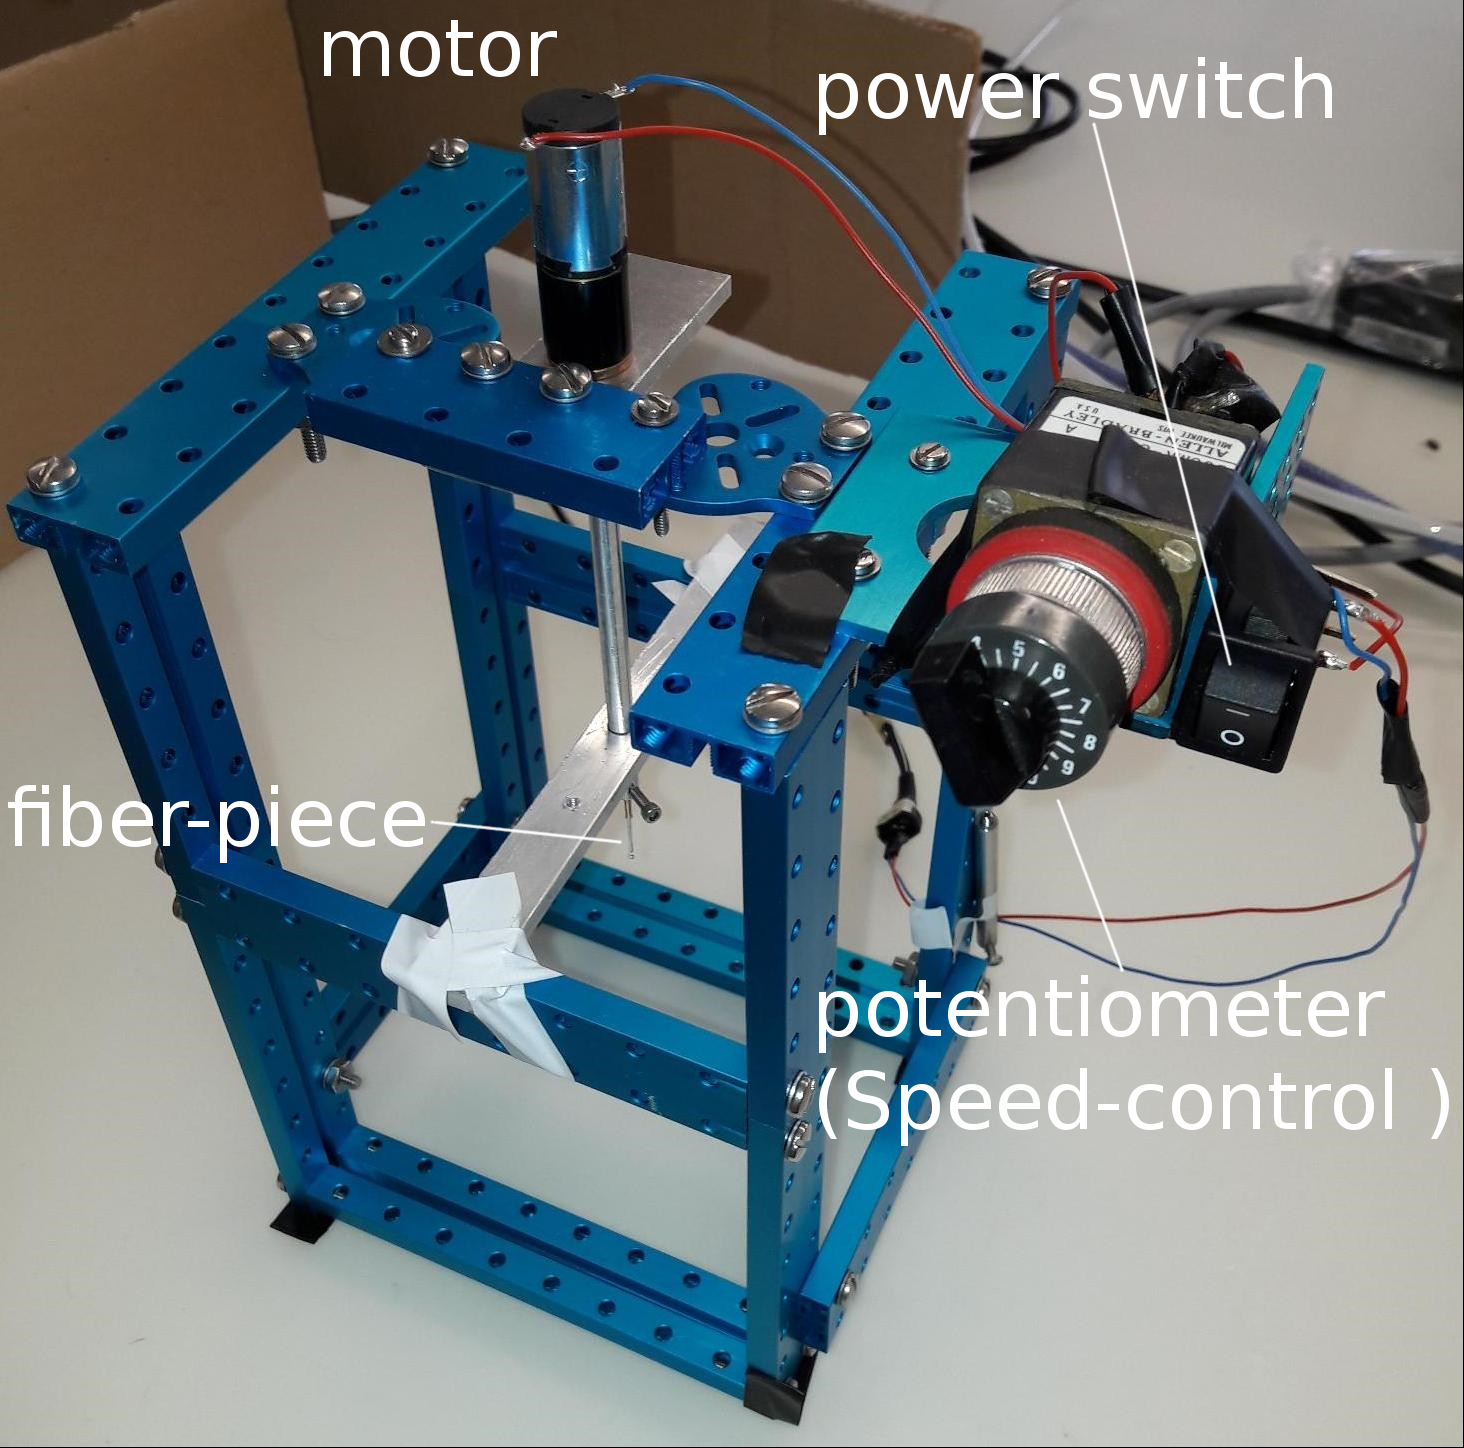
\includegraphics[scale=0.3]{source/melting_machine}
	\caption{A picture of the machine used for melting the glass rods. The framing is made from a construction kit from Makeblock. Some parts of the framing are custom made parts made from aluminum. The motor is from Maxxon (870 rpm, $41 \si{Nmm}$).}
	\label{Fig:Melting_machine}
\end{figure}
Without the spinning at approximately $11.4\si{Hz}$ (would be around $14.5\si{Hz}$ without the straightening fixture around the axles) the drop would not form a sphere in a controlled manner. \autoref{Fig:Melting_nonrotating} shows schematically how the formation without the spinning motion would look.
\begin{figure}[H]
	\includesvg[scale=0.3]{source/melting_nonrotating}
	\caption{Schematic depiction of a drop melted without the rotating motion during the process.}
	\label{Fig:Melting_nonrotating}
\end{figure}
With the machine shown in \autoref{Fig:Melting_machine} this problem can be omitted and the radius of the drop can be controlled by varying the speed of the machine and also by holding the blowtorch at different heights.
\begin{figure}[H]
	\includesvg[scale=0.3]{source/melting_rotating}
	\caption{Schematic depiction of the melting process with rotating axis.}
\end{figure}
For melting we used two different process gases: Acetylene at a pressure of $0.4\si{bar}$ and Oxygen at a pressure of $0.2\si{bar}$. To prevent soot from contaminating the stamp it is important to add Oxygen to the Acetylene flame. If the yellow in the flame disappears and a blue glow is emitted from the center of the flame the blowtorch has the right settings. The melting then simply takes place by holding the flame of the blowtorch to the rotating glass cylinder at approximately four millimetres above the lower end and waiting for the glass to melt and expand into a sphere. The blowtorch can then be turned off and in a short amount of time the glass cools down and forms a transparent sphere at the lower end of the cylinder.
\begin{figure}[H]
	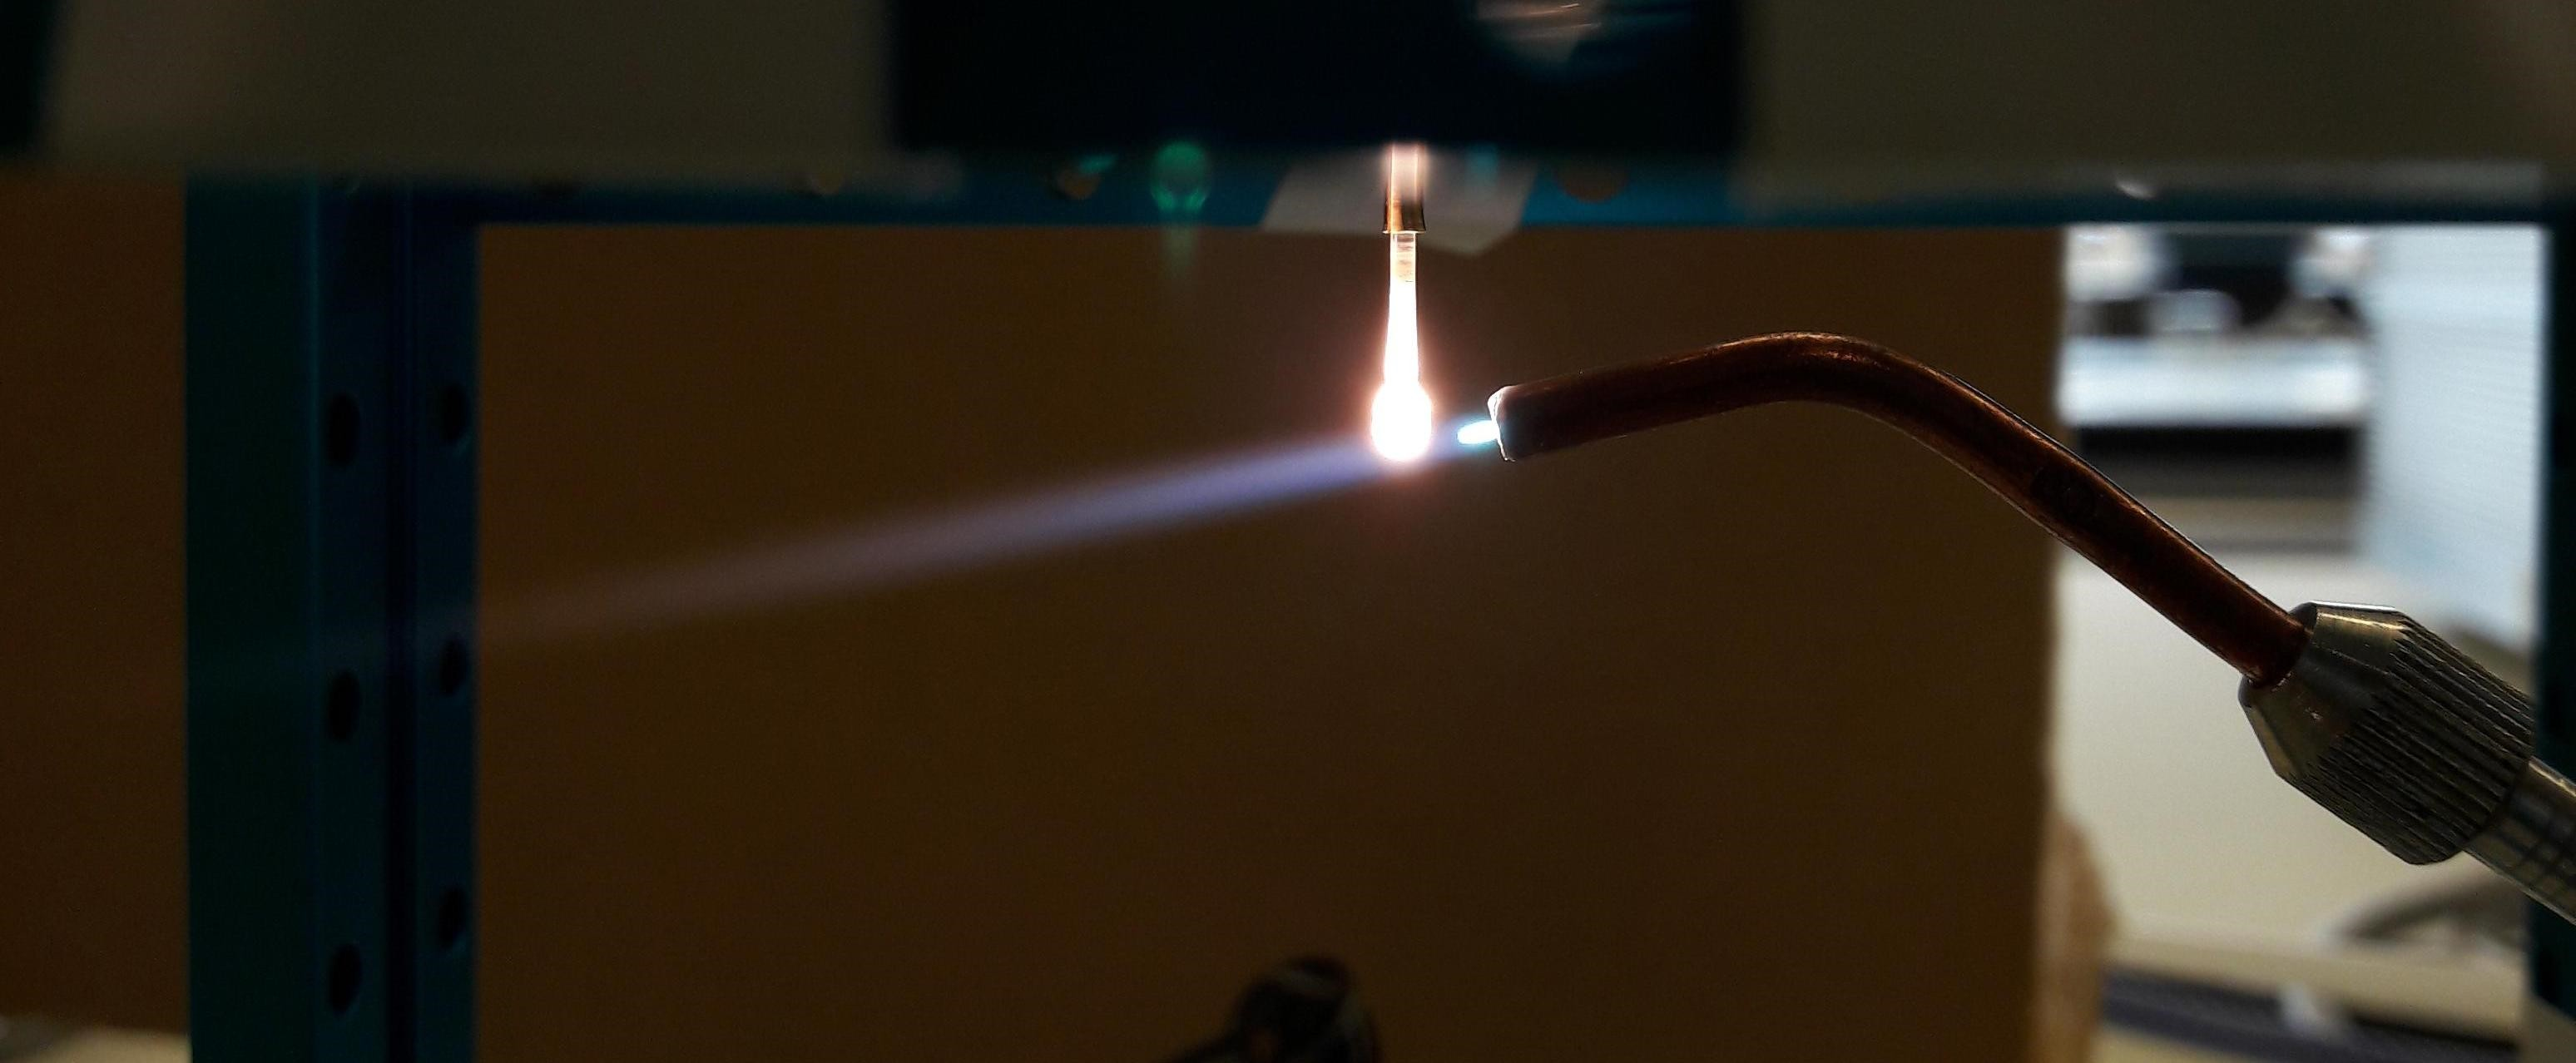
\includegraphics[scale=0.13]{source/melting}
	\caption{In this picture it can be seen how the rotating glass rod forms a drop which is spherical in the front. After cooling the surface is smooth [ref] and the stamp can be further processed.}
\end{figure}

\subsection{Measurement}
After the stamps have been fabricated by melting the extracted glass cylinders it is important that each one of them is being measured. It is necessary to know the radius of the spherical shape at the front very accurately to determine how large the diameter of the mirror will be and how deep it will be after imprinting. For this purpose the stamps are fixed inside a quartz-dish and photographed with a microscope. From this image a software developed in python can determine the radius of the spherical region that will be used as the actual stamp.

\begin{figure}[H]
	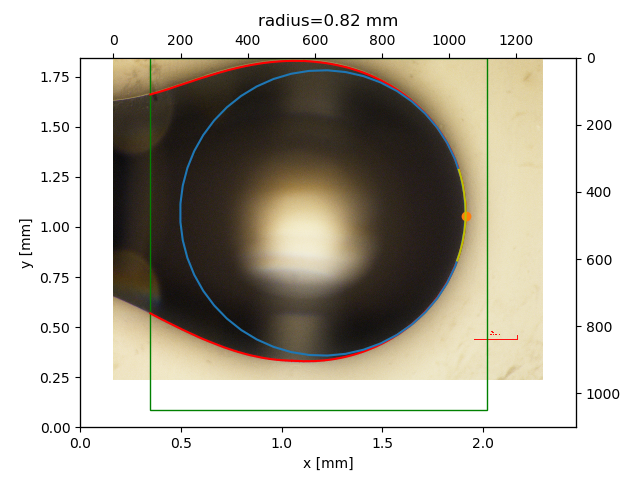
\includegraphics[scale=0.6]{source/radius_analysis}
	\caption{The software that is used for extracting the radius is developed in python. It is able to determine the orientation of a sample and uses this to predict which part of the stamp will be in contact with the polymer (marked yellow). The contact region is then used to extract the radius with at this position with the Ransac (Random sample consensus) [ref] algorithm.}
\end{figure}
From the radius we can then infer the dimensions of the actual mirror. First we need the beam waist radius in the focus so we can calculate the Rayleigh range. The wavefront radius is now fixed since the stamp is already fabricated and the cavity length we choose to be $500\si{\micro m}$ as discussed in \autoref{ChapCavityLength}. The following formula for the beam waist radius in the focus can be found by plugging \autoref{EqRayleighRange} into \autoref{EqWfRadius}:
\begin{equation}
	w_0(R, L)=\sqrt{\frac{\lambda}{\pi}}\left(L(R-L)\right)^{1/4}
\end{equation}


[Talk about the measured radii and the standard deviation]
[Talk about the methods to extract the mirror parameters from the radius]
\subsection{Silanization}
\subsection{Coverslip preparation}
\subsection{Mirror imprinting}
\subsection{Grinding}
\subsection{Cleaning}
\subsection{Coating}
\section{Analysis}